% ---------------------------------------------------------------------- %

\documentclass[letterpaper,10pt]{article}



\pagestyle{empty}

\usepackage[table]{xcolor}
\usepackage{color, colortbl}
\usepackage{tabularx}
\usepackage{amssymb}
\usepackage{enumerate}

\definecolor{LightGray}{gray}{0.9}

\usepackage{amsmath}
\usepackage{amscd}
\usepackage{url}

\usepackage{graphicx}


\title{Picking Travel Times}
\author{Seismo Group}
\date{\today}

\begin{document}
\maketitle

% ************************************************************* %
%                                                               %
%                       PICK TRAVEL TIMES                       %
%                                                               %
% ************************************************************* %

\section{Picking travel times}

In the terminal, cd into the directory with all the pkl files you want to run, and then do \verb"ttpick.py ___.bhz.pkl". You want to run either the \verb".bht" or \verb".bhz" files. 

A GUI should pop up if you successfully ran it.  

\begin{figure}[h!]
  \centering
  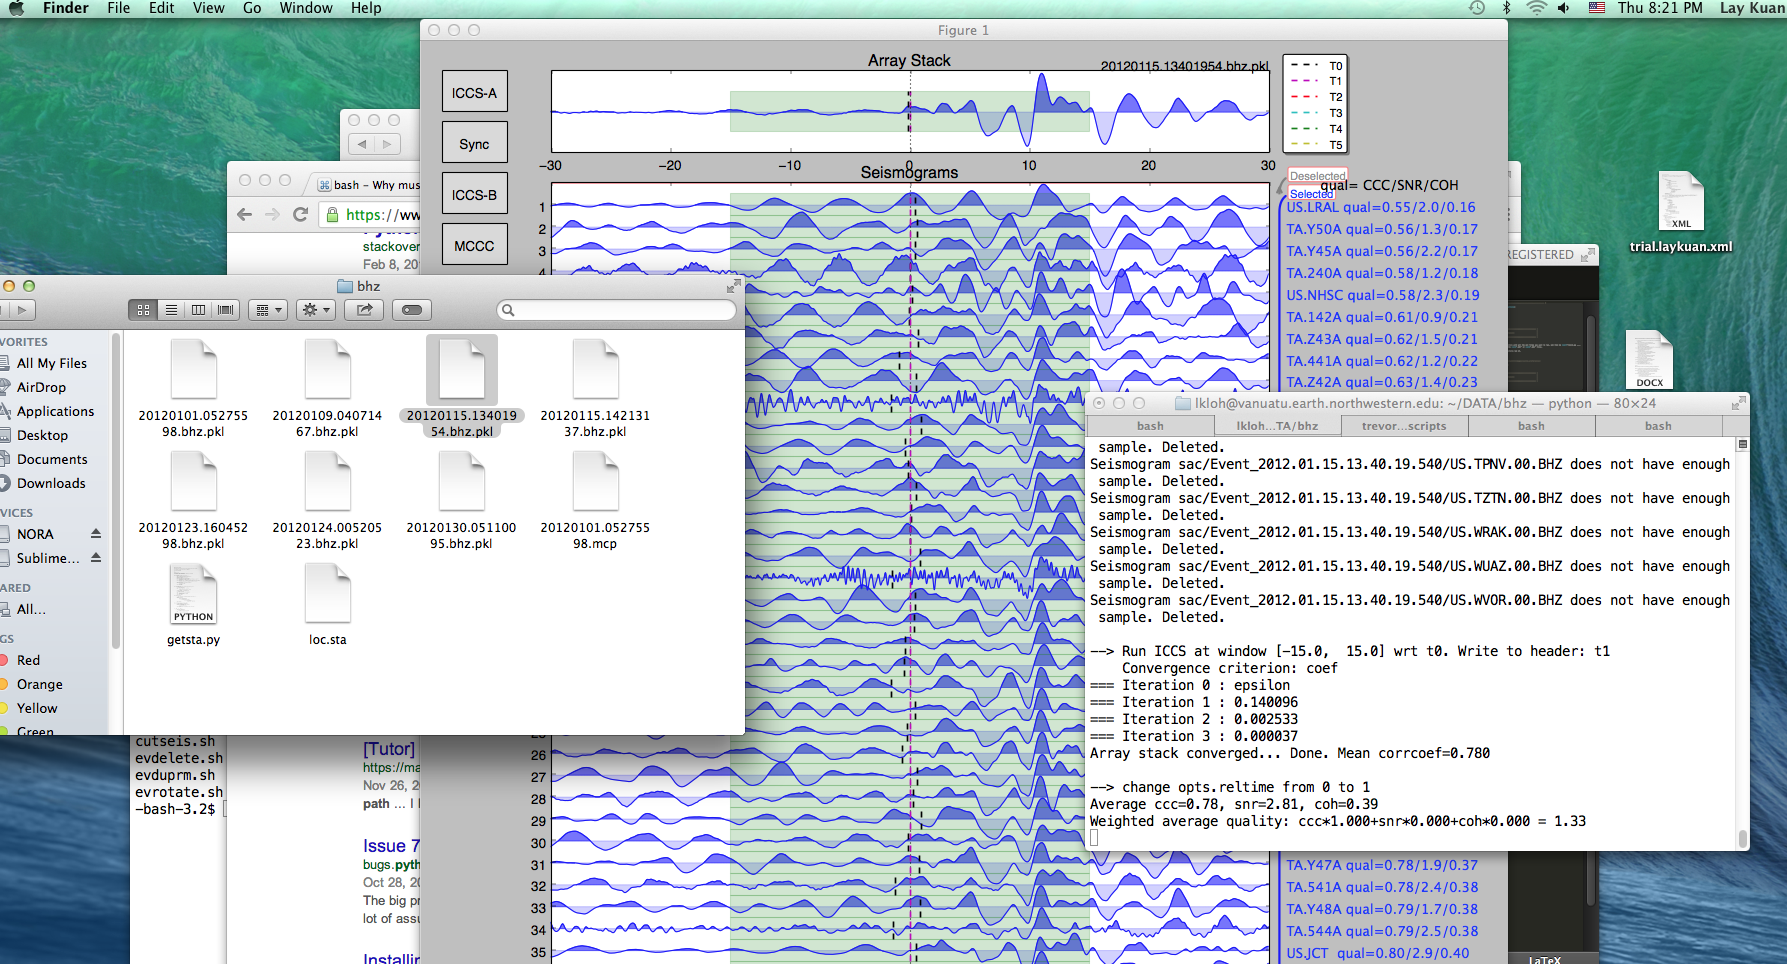
\includegraphics[width=0.5\textwidth]{images/pick_travel_times}
  \caption{Pick travel times}
  \label{fig:pick_travel_times}
\end{figure}

Remember to save your work periodically once you start picking your travel times, otherwise if AIMBAT crashes, you lose it. 


% ************************************************************* %
%                                                               %
%                       PICK TRAVEL TIMES                       %
%                                                               %
% ************************************************************* %



\end{document}

% --------------------------------- END --------------------------------- %
